\documentclass[]{politex}

% ========== Opções ==========
% pnumromarab - Numeração de páginas usando algarismos romanos na parte pré-textual e arábicos na parte textual
% abnttoc - Forçar paginação no sumário conforme ABNT (inclui "p." na frente das páginas)
% normalnum - Numeração contínua de figuras e tabelas 
%	(caso contrário, a numeração é reiniciada a cada capítulo)
% draftprint - Ajusta as margens para impressão de rascunhos
%	(reduz a margem interna)
% twosideprint - Ajusta as margens para impressão frente e verso
% capsec - Forçar letras maiúsculas no título das seções
% espacosimples - Documento usando espaçamento simples
% espacoduplo - Documento usando espaçamento duplo
%	(o padrão é usar espaçamento 1.5)
% times - Tenta usar a fonte Times New Roman para o corpo do texto
% noindentfirst - Não indenta o primeiro parágrafo dos capítulos/seções


% ========== Packages ==========
\usepackage[utf8]{inputenc}
\usepackage{amsmath,amsthm,amsfonts,amssymb}
\usepackage{graphicx,cite,enumerate}


% ========== Language options ==========
\usepackage[brazil]{babel}
%\usepackage[english]{babel}


% ========== ABNT (requer ABNTeX 2) ==========
%	http://www.ctan.org/tex-archive/macros/latex/contrib/abntex2
%\usepackage[num]{abntex2cite}

% Forçar o abntex2 a usar [ ] nas referências ao invés de ( )
%\citebrackets{[}{]}


% ========== Lorem ipsum ==========
\usepackage{blindtext}

% ========= Math Symbols =========
\usepackage{amsmath}

\DeclareMathOperator*{\argmax}{arg\,max}
\DeclareMathOperator*{\argmin}{arg\,min}

% ========== Opções do documento ==========
% Título
\titulo{Chatbot para Perguntas e Respostas com Capacidade de Explicação}

% Autor
\autor{Gustavo Padilha Polleti}

% Para múltiplos autores (TCC)
%\autor{Nome Sobrenome\\%
%		Nome Sobrenome\\%
%		Nome Sobrenome}

% Orientador / Coorientador
\orientador{Prof. Dr. Fábio Gagliardi Cozman}
% \coorientador{Nome do coorientador (opcional)}

% Tipo de documento
%\tcc{Eletricista com ênfase em Sistemas Eletrônicos}
\tcc{de Computação}
%\teseDOC{Engenharia Elétrica}
%\teseLD
%\memorialLD

% Departamento e área de concentração
\departamento{Computação e Sistemas Digitais}
\areaConcentracao{Computação}

% Local
\local{São Paulo}

% Ano
\data{2019}




\begin{document}
% ========== Capa e folhas de rosto ==========
\capa
%\falsafolhaderosto
\folhaderosto


% ========== Folha de assinaturas (opcional) ==========
%\begin{folhadeaprovacao}
%	\assinatura{Prof.\ X}
%	\assinatura{Prof.\ Y}
%	\assinatura{Prof.\ Z}
%\end{folhadeaprovacao}


% ========== Ficha catalográfica ==========
% Fazer solicitação no site:
%	http://www.poli.usp.br/en/bibliotecas/servicos/catalogacao-na-publicacao.html


% ========== Dedicatória (opcional) ==========
%\dedicatoria{Dedicatória}


% ========== Agradecimentos ==========
%\begin{agradecimentos}

%\end{agradecimentos}


% ========== Epígrafe (opcional) ==========
\epigrafe{%
	\emph{``Epígrafe''}
	\begin{flushright}
		-{Computers are like Old Testament gods: lots of rules and no mercy.}- Joseph Campbell
	\end{flushright}
}


% ========== Resumo ==========
\begin{resumo}
O presente trabalho descreve o desenvolvimento de um chatbot capaz de explicar suas próprias respostas. Nesse sentido, representa uma grande avanço rumo a uma relação humano-computador mais transparente e eficaz. O seu objetivo consiste em apoiar todo processo educacional de um estudante da USP, desde a consolidação de sua grade até a elucidação de dúvidas sobre as disciplinas. 

O agente conversacional aqui exposto utilizará o \textit{Knowledge Embedding} de uma base de conhecimento de domínio semi-aberto para responder perguntas relacionadas a diversas áreas do conhecimento. No quesito de interpretabilidade, será usado o método XKE (\textit{Explainable Knowledge Embedding}) como base para a geração de explicações em linguagem natural.
%
\\[3\baselineskip]
%
\textbf{Palavras-Chave} -- Chatbot, Explanation, Knowledge Embedding, Machine Learning, Expert System.
\end{resumo}


% ========== Abstract ==========
%\begin{abstract}
%Abstract...
%
%\\[3\baselineskip]
%
%\textbf{Keywords} -- Word, Word, Word, Word, Word.
%\end{abstract}


% ========== Listas (opcional) ==========
\listadefiguras
\listadetabelas

% ========== Listas definidas pelo usuário (opcional) ==========
\begin{pretextualsection}{Lista de Abreviações e Acrônimos}

\begin{flushleft}
USP \:\:\:\:\:\:\:\:\: Universidade de São Paulo \\
IA \:\:\:\:\:\:\:\:\:\:\:\:\: Inteligência Artificial \\
NLP \:\:\:\:\:\:\:\:\: Natural Language Processing \\
KB \:\:\:\:\:\:\:\:\:\:\:\: Knowledge Base \\
KE \:\:\:\:\:\:\:\:\:\:\:\: Knowledge Embedding \\
GUI \:\:\:\:\:\:\:\:\:\: Graphic User Interface \\
CLI \:\:\:\:\:\:\:\:\:\:\, Command Line Interface \\
CUI \:\:\:\:\:\:\:\:\:\: Conversational User Interface \\
GCP \:\:\:\:\:\:\:\:\, Google Cloud Platform \\
LIME \:\:\:\:\:\:\: Local Interpretable Model-Agnostic Explanations \\
XKE \:\:\:\:\:\:\:\:\: Explainable Knowledge Embedding \\
GPU \:\:\:\:\:\:\:\:\: Graphics Processing Unit \\
TP \:\:\:\:\:\:\:\:\:\:\:\:\: True Positive  \\
FP \:\:\:\:\:\:\:\:\:\:\:\:\: False Positive \\
FN \:\:\:\:\:\:\:\:\:\:\:\:\: False Negative \\
TN \:\:\:\:\:\:\:\:\:\:\:\:\: True Negative

\end{flushleft}

\end{pretextualsection}

% ========== Sumário ==========
\sumario



% ========== Elementos textuais ==========

\part{Introdução}
	
\chapter{Introdução}
\capepigrafe[0.5\textwidth]{``Man is a political animal. A man who lives alone is either a Beast or a God.''}{Aristóteles}

O homem é um animal político. Na obra \textit{Política}, Aristóteles propõe que a natureza humana tem como aspecto fundamental a vida em sociedade. A natureza, como costuma-se dizer, nada faz em vão, e o homem é o único animal dotado por ela com o dom da fala. Enquanto a mera voz é nada mais do que um indicador de prazer ou dor, e portanto encontrada em outros animais, o poder da fala tem o propósito de separar o justo do injusto, o bom do mau \cite{aristotlePolitcs1905}. A capacidade e a necessidade de se comunicar com os demais para compartilhar sua visão de mundo  representa a base do que é ser humano.

O dom de se comunicar com seu semelhante, na visão aristotélica, diferencia o ser humano dos demais e, assim, confere a ele uma posição mais elevada. Tal capacidade de dialogar pode ser entendida como uma manifestação muito significativa de inteligência. O próprio Aristóteles, na obra \textit{Ética a Nicômaco}, afirma que o homem é um animal racional, pois, independente das suas individualidades, todos compartilham um senso comum de justiça e razão \cite{aristotle_2000}. 

Ao considerar esse aspecto mais básico do que caracteriza a humanidade, é inevitável que surjam questões como: a fala e a razão são exclusivos do ser humano? Ou é possível reproduzir tais atributos de modo a criar uma inteligência artificial?

Desde seu alvorecer, a humanidade sonha em criar inteligência. Por exemplo, na Grécia Antiga, personagens míticos como Pigmaleão e Hefesto, os quais podem ser interpretados como os inventores lendários de Galatea e Pandora, suas respectivas máquinas dotadas de razão, já aparecem na cultura e na filosofia Ocidental  \cite{Goodfellow-et-al-2016}. No século XX, a partir dos progressos na ciência da computação, esse sonho começa a tomar forma com o jogo da imitação, teste postulado por Alan Turing que propõe a simulação do diálogo com um ser humano como prova de inteligência.

Atualmente, esse sonho assume a forma de agentes conversacionais, os quais estão cada vez mais presentes e atuantes na sociedade contemporânea. Em geral, suas funções são simples e bem objetivas, como realizar reservas em restaurantes, informar a previsão do tempo, enviar emails, etc, apesar de que existem outros contextos mais complexos. Por exemplo, inserido no ambiente do IoT (\textit{Internet das Coisas}), o agente da Amazon, Alexa, já é amplamente utilizado em automação residencial e, hoje, já transforma o estilo de vida de várias famílias no mundo inteiro \cite{Sciuto:2018:HAW:3196709.3196772}. Também, o assistente virtual Siri, da Apple, está presente em 44\% de todos os smartphones em 2018 e está sendo usado diariamente para tarefas, desde realizar chamadas até funções de entretenimento \cite{assistantStats}. As possibilidades de aplicação são inúmeras e o real impacto dessa tecnologia só poderá ser medido nos próximos anos, porém os desafios são igualmente significativos.

Embora ainda não seja possível reproduzir fielmente, no sentido mais geral, o raciocínio humano, os avanços na área são realmente notáveis. O progresso em NLP (\textit{Processamento de Linguagem Natural}) permitiu a computação eficaz da semântica em texto, o que por sua vez abriu espaço para a identificação de intenções e tradução automática. Desse modo, uma máquina seria capaz de tratar uma mensagem não estruturada ou com sentidos mais abstratos. Também, vale ressaltar como as recentes técnicas de Aprendizado Profundo, especialmente no que tange à redes neurais recorrentes e LSTMs, tornaram possível a geração de texto com qualidade.

Todos esses avanços culminaram na situação em que uma máquina consegue processar, entender e gerar texto de forma inédita na história da inteligência artificial. Porém, o que essas técnicas avançadas, com destaque para Aprendizado Profundo, trazem de benefício em termos de acurácia, perdem em interpretabilidade. Por exemplo, quanto mais complexo é um modelo, mais eficientemente ele descreve um comportamento, porém ao mesmo tempo se torna tão complexo a ponto de um ser humano não ser mais capaz de entendê-lo.

Isso acaba por limitar sua aplicação a situações de baixo risco. Por exemplo, é factível um agente conversacional cuja função é recomendar filmes, pois, o pior caso seria o usuário desperdiçar algumas horas em um conteúdo que não o agrade. Porém, caso o agente conversacional informe a autorização de uma linha de crédito, qualquer erro ou até mesmo um desentendimento pode impactar muito negativamente. Nesse último caso, é fundamental que, além de informar a decisão, o sistema também explique o resultado. Inclusive, alguns governos tornaram o direito à explicação uma obrigação legal de empresas que utilizem sistemas automáticos de tomada de decisão \cite{eu-269-2014}.

Assim como o cientista Alan Turing afirmou em \textit{"We can only see a short distance ahead, but we can see plenty there that needs to be done"}, existe muito trabalho a ser realizado antes do dia em que se terá uma inteligência artificial comparável ao intelecto humano. Tarefas mais avançadas que exigem transparência em seu raciocínio e, ao mesmo tempo, alta acurácia são realmente desafiadoras.  

Inserido nesse cenário, este trabalho busca ampliar as fronteiras de aplicação dos agentes conversacionais para casos de uso mais complexos. Se até agora, as máquinas foram capazes de responder os "O que?", "Quando?" e "Onde?", este trabalho irá capacitá-las a responder também o "Por quê?".

\section{Objetivo}

O objetivo deste trabalho é projetar e desenvolver um chatbot capaz de assessorar estudantes da USP ao longo de seu ciclo de vida universitário, ou seja, desde a consolidação de sua grade curricular até a elucidação de dúvidas pontuais. A proposta é proporcionar ao aluno a melhor experiência de ensino ao facilitar a busca de conteúdos e informações que contribuam ao seu aprendizado.

Este trabalho dará continuidade  a um projeto de formatura concluído em 2018 \citebrackets{(Correa-et-al-2018)}, o qual também contou com a orientação do Prof. Fabio Cozman \cite{Correa-et-al-2018}. Nesse trabalho de referência, além da arquitetura base, serão aproveitados alguns aspectos da análise de tecnologias relacionadas e as métricas de avaliação.

A princípio, o chatbot a ser desenvolvido será voltado a perguntas e respostas sobre sistema Júpiter de gestão da graduação da USP \footnote{acesso via https://uspdigital.usp.br/jupiterweb/}. Esse sistema contém uma quantidade significativa de informações e é de vital importância para os estudantes da USP. Considere o exemplo de diálogo abaixo:

\begin{flushleft}
    \textit{Usuário:} Quais os oferecimentos para a disciplina Aprendizado Estatístico? \\
    \textit{Chatbot:} O curso é oferecido das 09:00 am até as 12:00 às Terças-feiras.
\end{flushleft}

Além de sanar dúvidas e buscar informações relativas aos cursos oferecidos na universidade, por exemplo \textit{"Qual os horários de oferecimento da disciplina XYZ?"}, deve ser capaz de recomendar disciplinas e materiais de estudo (artigos) baseados no interesse do estudante. Vale ressaltar a importância de cada sugestão conter uma ou mais razões a fim de aumentar a confiança do usuário na recomendação. Considere o exemplo abaixo:

\begin{flushleft}
    \textit{Usuário:} Quais as disciplinas sobre Redes Neurais me sugere? \\
    \textit{Chatbot:} Recomendo Aprendizado Estatístico, pois trata de Inteligência Artificial.
\end{flushleft}

A explicação "\textit{... pois trata de Inteligência Artificial}" fortalece a recomendação, pois indica ao usuário de que tanto o tema \textit{"Redes Neurais"} como a disciplina \textit{Aprendizado Estatístico} estão relacionadas com o assunto \texit{Inteligência Artificial}.

Por fim, também deve auxiliar o aluno durante o processo de aprendizado ao responder e explicar possíveis dúvidas sobre os conteúdos estudados. Considere o exemplo de diálogo abaixo:

\begin{flushleft}
    \textit{Usuário:} Interpretabilidade em IA é importante? \\
    \textit{Chatbot:} Sim, pois não se pode confiar no que não se entende.
\end{flushleft}

Neste caso, a explicação tem papel central, isto é, de nada serviria a resposta "\texit{Sim}" sem o complemento. O processo de ensino essencialmente consiste em um raciocínio explicativo, no qual o aprendizado se dá justamente ao relacionar conceitos previamente conhecidos com novos ou no estabelecimento de novas relações. Além de que é possível encontrar na literatura casos em que explicações contribuíram para uma melhor experiência de aprendizado. \cite{DBLP:conf/iui/PutnamC19}

O chatbot deve ser flexível o bastante para tratar mensagens não-estruturadas, ou seja, identificar as intenções em mensagens para as quais não foi previamente treinado. Desse modo, deve conseguir lidar com a linguaguem coloquial típica do ambiente universitário, além de lidar com erros ortográficos, abreviações e sinônimos.

\section{Motivação}

O projeto Jupiterweb Bot comprovou a viabilidade de se aplicar um chatbot no contexto universitário, por meio de pesquisas de satisfação e entrevistas com os usuários \cite{Correa-et-al-2018}. Isto posto, a principal motivação deste trabalho é dar continuidade ao projeto de referência com o mesmo intuito de facilitar a vida do estudante da USP e, assim, proporcionar a melhor experiência de aprendizado possível. 

Ao mesmo tempo, espera-se contribuir para o desenvolvimento de chatbots com real habilidade de interagir com humanos em diálogos complexos. A capacidade de explicar decisões é fundamental em tais interações, e este projeto dará os passos iniciais para se atingir tal aptidão.

\section{Estado da Arte}

Os primeiros chatbots funcionais se baseavam na mera decomposição das frases recebidas em palavras-chave, cuja presença causavam o acionamento de regras pré-definidas. Um exemplo bem conhecido é o ELIZA \cite{Weizenbaum:1966:ECP:365153.365168}. Apesar de ser muito simples, consegue apresentar um comportamento de indagação recursiva, isto é, a cada iteração, responde o usuário com um questionamento flexível a vários contextos, o que permite diálogos relativamente longos. 

A principal limitação de ELIZA está na ausência de técnicas mais avançadas de processamento de linguagem natural, o que impossibilita uma análise semântica da frase. Nesse sentido, o chatbot não consegue capturar os elementos e as suas relações em cada contexto nem identificar erros de digitação. Além de que não é capaz de lidar com várias intenções em uma mesma frase, nesses casos acionará uma única regra e descartará as demais.

Desde a ELIZA, os agentes conversacionais tiveram enorme progresso, e hoje conseguem realizar a interface humano-computador de forma convincente. Alguns são projetados para simular conversas curtas, com foco em busca de informações; exemplos como Cortana e Alexa já estabeleceram sua presença na sociedade. Os comumente designados ``chatbots", por sua vez, são mais abrangentes, uma vez que visam sustentar interações complexas com texto pouco ou nada estruturado e frequentes transições de assuntos \cite{Bollacker:2008:FCC:1376616.1376746}. 

O qualidade do diálogo, analisado como uma tarefa de NLP, é bem difícil de ser avaliada, a abordagem mais comum envolve avaliação humana. O diálogo pode ser dividido em três áreas principais: \textit{Dialogue Act Classification}, \textit{Dialogue State Tracking} e \textit{Retrieval-based Chatbot}.

\subsection{Dialogue Act Classification}

O DAC (\texit{Dialogue Act Classification}) é um desafio relacionado à interpretação do diálogo, cujo objetivo consiste em classificar sentenças segundo a intenção do usuário. Por exemplo, a sentença "\textit{Olá, tudo bem?}" poderia ser rotulada com a intenção "\textit{Saudação}". Dessa forma, pode-se modelar e estruturar o diálogo. 

Agentes conversacionais, de forma geral, se beneficiam muito de \textit{Dialogue Act Classification}. O DAC pode ser utilizado de modo a proporcionar conversas orientadas à tarefas, o que por sua vez tem ampla aplicação em chatbots e assitentes virtuais. 

Os melhores resultado em DAC, até o momento, foram obtidos em 2018 com a técnica \textit{Conditional Random Fields - Attentive Network} \cite{DBLP:journals/corr/abs-1711-05568}. Esse método se apropria da ideia de que o histórico de sentenças e seus rótulos podem contribuir para uma melhor classificação, o que é bem intuitivo pois em um diálogo a sequência de mensagens costuma estar relacionada. Nesse sentido, são utilizadas redes neurais recorrentes bidirecionais composta por unidades biGRU (\textit{Gated Recurrent Unit}).  

\subsection{Dialogue State Tracking}

O DST (\textit{Dialogue State Tracking}), o qual consiste no desafio em estimar o estado dos objetivos e requisições do usuário no contexto do diálogo, é uma parte essencial de sistemas conversacionais orientados a tarefas. O seu propósito é planejar a próxima ação ou resposta pela análise do histórico da conversa mais a última mensagem.

Em 2018, foi proposto o GLAD (\textit{Global-Locally Self-Attentive Dialogue Tracker}) \cite{DBLP:journals/corr/abs-1805-09655}, o qual aprende representações tanto das mensagens do usuário como das ações passadas do sistema a partir de módulos globais e locais. Essa abordagem se mostrou bem sucedida em capturar estados raros e, assim, atingiu performance superior.  

\subsection{Retrieval-based Chatbot}

Um grande desafio na área de agentes conversacionais é a \textit{Response Selection}. Dada uma pergunta do usuário, além de um chatbot enfrentar a dificuldade de encontrar a resposta correta, em geral, existem várias respostas possíveis e selecionar a mais apropriada é uma tarefa nada trivial. Por exemplo, considere o diálogo abaixo:

\begin{flushleft}
    \textit{Usuário:} Por que o meu vôo foi cancelado? \\
    \textit{Chatbot:} Por que a válvula de descompressão XYZ apresentou ABCD. 
\end{flushleft}

No exemplo acima, a resposta do chatbot só seria adequada caso o usuário seja um engenheiro que conheça os detalhes técnicos de funcionamento de um avião. Porém, pelo teor da pergunta, é provável que seja um passageiro leigo no assunto, logo, a explicação densa em detalhes técnicos pouco ou nada contribuiu para seu entendimento.

O estado da arte é uma abordagem baseada em \textit{Transformer Neural Network}, desenvolvida em 2017, que propõe a seleção da resposta em função de seu grau de correspondência com a pergunta \cite{P18-1103}. Uma resposta teria mais preferência caso seus termos também estejam presentes na pergunta, por exemplo.

\section{Justificativa}

Em vista da atual perspectiva de atendimento de forma bem eficiente, vários pacotes de desenvolvimento de chatbots foram recentemente lançados (por exemplo, IBM Watson, Microsoft BotKit, Wit.ai, Dialogflow). Estes pacotes permitem a definição de contextos, dados de treino, exemplos de respostas e mensagens de erro, o que os tornam bastante flexíveis. No entanto, as ferramentas hoje disponíveis têm claras limitações. Uma restrição é o incipiente suporte de ontologias. Uma ontologia oferece relacionamentos semânticos entre os termos, além de ser útil para auxiliar em buscas -- por exemplo, um chatbot pode perguntar a um paciente se a dor é no tórax ou na cabeça e ficar satisfeito com a resposta ``na orelha", ao reconhecer que é uma parte da cabeça por meio de uma ontologia médica \cite{MilwardBeveridge03KRPDS}.

Um outro ponto que recebe pouco ou até mesmo nenhum suporte em plataformas para chatbots é a geração de explicações. Embora a pesquisa em aprendizado de máquina tenha, recentemente, demonstrado interesse em explicar decisões automáticas \cite{Ribeiro:2016:WIT:2939672.2939778}, ainda não se encontram na literatura resultados sobre interpretabilidade em chatbots. 

Para entender o desafio imposto pela geração de explicações durante um diálogo, considere um exemplo:

\begin{flushleft}
    \textit{Usuário:} Existe a possibilidade de investir no tesouro direto? \\
    \textit{Chatbot:} Não é possível oferecer esse serviço. \\
    \textit{Usuário:} Por quê?
\end{flushleft}

Qual seria a explicação adequada? Informar uma razão muito técnica, como ``Porque o regulamento XYZ do Banco Central não permite", não seria adequada para um usuário leigo. Talvez uma resposta um pouco mais adequada seria: ``Porque na sua faixa de renda isso não é possível", porém essa explicação não oferece nenhuma orientação sobre como o usuário deve proceder para atingir seu objetivo de investimento. Nesse sentido, seria ainda mais apropriada uma resposta como: ``Se sua renda mensal não fosse menor do que R\$X seria possível investir." Para emitir tal explicação, o sistema precisa lidar com o contexto do usuário e com as regras do domínio de interesse.

Como um segundo exemplo, considere um chatbot que responde perguntas genéricas a partir de consultas a uma base de conhecimento de grande porte, como por exemplo a Freebase \cite{Bollacker:2008:FCC:1376616.1376746}. Considere o diálogo:

\begin{flushleft}
    \textit{Usuário:} O rei Francisco II das Duas Sicílias foi católico? \\
    \textit{Chatbot:} Sim. \\
    \textit{Usuário:} Por quê?
\end{flushleft}

Essa informação não está disponível na Freebase, a explicação não é trivial e, portanto, precisa ser concluída a partir de outros fatos presentes na base de conhecimento. Conforme discutido em artigo publicado pelo grupo de pesquisa do orientador, pode-se extrair automaticamente a seguinte razão: "Pois seus pais e esposa foram católicos" \cite{DBLP:journals/corr/abs-1806-09504}

Tal capacidade de gerar explicações é desejada em vários casos, especialmente no suporte à tomada de decisão, como em sistemas de recomendações. Nesses casos, a eficácia do sistema depende fortemente do grau de confiança que o usuário deposita nas sugestões. Por exemplo, dada a recomendação de uma marca de vinho, a chance de comprar ou não o destilado depende do quanto se crê no bom gosto de quem a sugeriu. Nesse sentido, apresentar as razões que levaram a uma decisão contribuem para elevar sua credibilidade \cite{molnar2019}.

Com esse propósito, existe um esforço da academia no sentido de construir \textit{transparente recommendation systems} \cite{Musto-et-al}. Nesse trabalho foi desenvolvido um sistema de recomendação conversacional com capacidade de explicação. 

Além da academia, a sociedade como um todo tem demonstrado grande preocupação com essas questões, o que se traduz em medidas regulatórias que assegurem ao cidadão o direito à explicação. Legislação como o GDPR \cite{eu-269-2014} e a lei de proteção de dados no Brasil são importantes pois, ao exigir interpretabilidade dos sistemas automáticos de decisão, que cada vez mais são completas caixas-pretas, consegue-se mitigar problemas de viés e, é garantida uma relação mais transparente e justa entre todas as partes. 

\section{Organização do Trabalho}

Este trabalho é apresentado de acordo com o modelo padrão de projeto de formatura. Dessa forma, foi dividido em outras 4 partes:

\begin{enumerate}
    \item \textbf{Aspectos Conceituais} \\
    Nesta parte é exposta uma explicação geral e básica sobre os principais temas do trabalho, como forma de contextualização. 
    \item \textbf{Tecnologias Utilizadas} \\
    Aqui são apresentadas a seleção de tecnologias integradas no projeto final, bem como as razões para sua escolha.
    \item \textbf{Metodologia de Projeto} \\
    Introduz de forma resumida as diretrizes adotadas para este projeto e a sequência de atividades planejadas.
    \item \textbf{Especificação e Requisitos do Sistema} \\
    Apresenta a especificação e os requisitos de forma detalhada, inclusive diagramas e demais formas de documentação.
\end{enumerate}

Como esta é uma versão inicial do trabalho, não são incluídas as partes: Projeto e Implementação, Avaliação e Teste, e Considerações finais. 

\part{Aspectos Conceituais}

\chapter{Aspectos Conceituais}
\capepigrafe[0.5\textwidth]{``If I have seen further than others, it is by standing upon the shoulders of giants.''}{Sir Isaac Newton}

Os aspectos conceituais expostos nesta seção buscam contextualizar este projeto nas grandes áreas de Inteligência Artificial, Engenharia de Software e Interação Homem-Máquina. 

\section{Explainable Artificial Intelligence (XAI)}

Se no passado, as grandes dificuldades para o progresso da Inteligência Aritificial residiam na pouca capacidade de processamento e na carência de dados. Com o poder computacional acessível pelas plataformas de nuvem (e.g. AWS, GCP, Azure, etc) e com as imensas quantidades de dados não estruturados disponíveis (\textit{Big Data}), essas antigas complicações são muito menos significantes. Isso proporcionou a aplicação de IA nas mais diversas indústrias, desde o entretenimento até o mercado financeiro. Porém, hoje surge uma nova barreira tão ou até mais desafiadora, a da interpretabilidade.

O principal problema por trás da necessidade de interpretação é a insuficiência de uma única métrica, como a acurácia, descrever a maioria das tarefas do mundo real \cite{2017arXiv170208608D}. Interpretabilidade e explicabilidade tem papel crucial em facilitar o aprendizado, satisfazer a curiosidade humana \cite{molnar2019} e, acima de tudo, criar confiança na relação humano-computador. Assim, é muito difícil atingir um bom grau de aceitação social sem que os processos de decisão automática sejam inteligíveis.

\subsection{Ética da Inteligência Artificial}

Modelos de aprendizado de máquina estão sujeitos a assimilar algum aspecto imoral latente em seu dataset, o que pode gerar predições racistas, sexistas ou imparciais completamente indesejadas. Em 2015, fontes tanto da mídia como da academia reportaram um aparente viés de gênero no Google search, nesse caso os principais resultados de uma busca de imagem para “CEO” mostravam somente homens brancos \cite{Yapo-et-al2018}. Pouco depois desse episódio, pesquisadores da Carnegie Mellon University revelaram que o Google apresentou seis vezes menos propagandas de emprego de cargos executivos para uma mulher do que para um homem que estivesse à procura de emprego \cite{Yapo-et-al2018}. 

Estes são exemplos de discriminação que derivado da falta de transparência. Técnicas avançadas, como \textit{Deep Learning}, apesar da alta performance dificulta a detecção de viés devido à sua baixa interpretabilidade.  Assim, conforme a presença da inteligência artificial cresce na sociedade moderna, também aumenta a preocupação de que aspectos como o viés acabe ferindo a ética ou até prejudiquem humanos \cite{Bostrom_theethics}.

\subsection{Taxonomia e Escopo da Interpretabilidade}

Com o propósito melhorar a interação da sociedade com sistemas que envolvem IA, a comunidade científica está mobilizada em desenvolver métodos capazes de aumentar a interpretabilidade. Tais esforços estão concentrados em métodos agnósticos a modelo, ou seja, técnicas passíveis de serem utilizadas em qualquer modelo, seja uma rede neural, floresta aleatória, etc.

Existem pelo menos duas definições subjetivas de interpretabilidade. A primeira é ``\textit{Interpretability is the degree to which a human can understand the cause of a decision}" \cite{DBLP:journals/corr/Miller17a}. A segunda é ``\textit{Interpretability is the degree to which a human can consistently predict the model’s result}" \cite{NIPS2016_6300}. Enquanto que a primeira busca uma explicação de escopo local, isto é, capaz de pontuar as causas de uma única previsão que já ocorreu (\textit{a posteriori}), a segunda adota uma abordagem global a fim de entender o modelo \texit{a priori}. Um exemplo de técnica explicação local agnóstica a modelo já utilizada comercialmente é o  \textit{Local-Surrogate} (LIME) \cite{Ribeiro:2016:WIT:2939672.2939778}.

\begin{figure}[h]
    \centering
    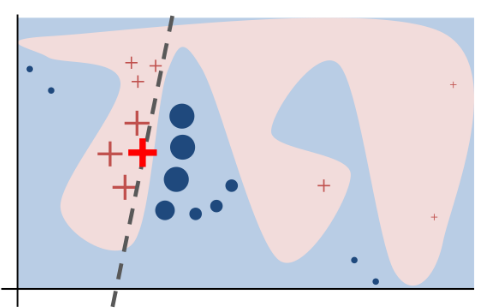
\includegraphics[width=0.6\textwidth]{images/lime-showcase.png}
    \caption{Explicação local de um modelo complexo por LIME \cite{Ribeiro:2016:WIT:2939672.2939778}.}
    \label{fig:lime_showcase}
\end{figure}

\subsection{Counterfactual Explanations}

A característica que talvez seja a mais importante de uma explicação é a sua \texit{human-friendliness}. Como já foi visto em exemplos anteriores, de nada adianta apresentar razões que, apesar de corretas, não tem significado para o usuário ou que são tão detalhadas a ponto de não serem inteligíveis. Desse modo, espera-se que uma boa explicação seja curta, esteja inserida no contexto social da conversa e, principalmente, seja contrastante \cite{molnar2019}. O contraste consiste em apresentar um exemplo, artificial ou não, no qual o evento em questão não teria ocorrido.

Por exemplo, considere o exemplo abaixo de uma explicação contrastante:

\begin{flushleft}
    \textit{Usuário:} Por que eu fui reprovado? \\
    \textit{Chatbot:} Se você não tivesse atrasado o trabalho final, você não teria sido reprovado. 
\end{flushleft}

Em termos práticos, uma explicação contrastante de uma predição descreve a menor mudança em uma situação que acarretaria na alteração da predição para um resultado pré-definido. No exemplo acima, o aluno é informado de que se pelo menos tivesse entregado o trabalho no prazo, seria aprovado na disciplina, isto é, teria atingido seu objetivo. 

Vale ressaltar que esse método é agnóstico a modelo e busca encontrar explicações locais. Em Wachter et. al (2017) \cite{DBLP:journals/corr/abs-1711-00399} é proposta como abordagem para geração de explicações contrastantes, a minimização da seguinte função de perda:

\begin{equation}
    L(x,\Acute{x},\Acute{y},\lambda)=\lambda⋅(\hat{f}(\Acute{x})- \Acute{y})^{2}+d(x,\Acute{x}).
\end{equation}

O primeiro termo da equação representa a distância quadrática entre a predição do modelo ($\hat{f}$) para o contrafactual $\Acute{x}$ e o \textit{target} $\Acute{y}$, o qual deve ser pré-definido. O segundo termo é a distância entre a instância $x$ e o contrafactual $\Acute{x}$. O parâmetro $\lambda$ pondera a distância na predição (primeiro termo) frente a distância nos valores das \textit{features}. Em outras palavras, um valor alto de $\lambda$ significa que é preferível um contrafactual próximo de $\Acute{y}$, enquanto um valor pequeno favorece aqueles bem similares a $x$.

Ao invés de otimizar essa função diretamente pelo $\lambda$, os próprios autores da técnica recomendam definir uma tolerância $\epsilon$ do quanto a predição do contrafactual pode se distanciar do resultado desejado. Observe essa restrição na relação abaixo:

\begin{equation}
    |\hat{f}(\Acute{x}) - \Acute{y}| \leq \epsilon.
\end{equation}

A função de perda é minimizada para $\Acute{x}$ e enquanto se aumenta o valor de $\lambda$ até se atingir uma solução suficientemente próxima, sempre dentro da tolerância $\epsilon$. 

\begin{equation}
    \arg\,\,\,\min_{\Acute{x}}\,\,\,\max_{\lambda}\,\,L(x, \Acute{x}, \Acute{y}, \lambda).
\end{equation}

A função $d$ da distância entre a instância $x$ e o contrafactual $\Acute{x}$ recomendada pelos autores do método é a distância Manhattan ponderada pela \textit{inverse median absolute deviation} (MAD).

\begin{equation}
    d(x, \Acute{x}) = \sum_{j=1}^p \frac{|x_{j} - \Acute{x_{j}}|}{MAD_j}.
\end{equation}

Com isso, é possível encontrar explicações baseadas em exemplos contrastantes e com alto grau de informação para o usuário. Essa técnica será a base para a geração de explicações do chatbot deste trabalho. 

\section{Knowledge Base}

Este tipo de base consiste em uma coleção de fatos, os quais podem ser descritos como uma relação entre duas entidades. Por exemplo a tripla $<$\textit{Aluno XYZ, Cursa, Engenharia}$>$ é uma forma de informação factual, na qual o \textit{Aluno XYZ} e \textit{Engenharia} são duas entidades e, \textit{Cursa} é o relacionamento entre elas. Vale reparar que a relação é unidirecional, isto é, o inverso não é necessariamente verdadeiro. 

Embora atualmente haja várias bases de conhecimento com bilhões de triplas, a incompletude ainda representa um grande desafio. Nesse sentido, existe um grande esforço da academia no desenvolvimento de técnicas que possibilitem, tanto deduzir novos fatos, como depurar essas bases para remover fatos falsos. \cite{journals/corr/NickelMTG15}

\begin{figure}[h]
    \centering
    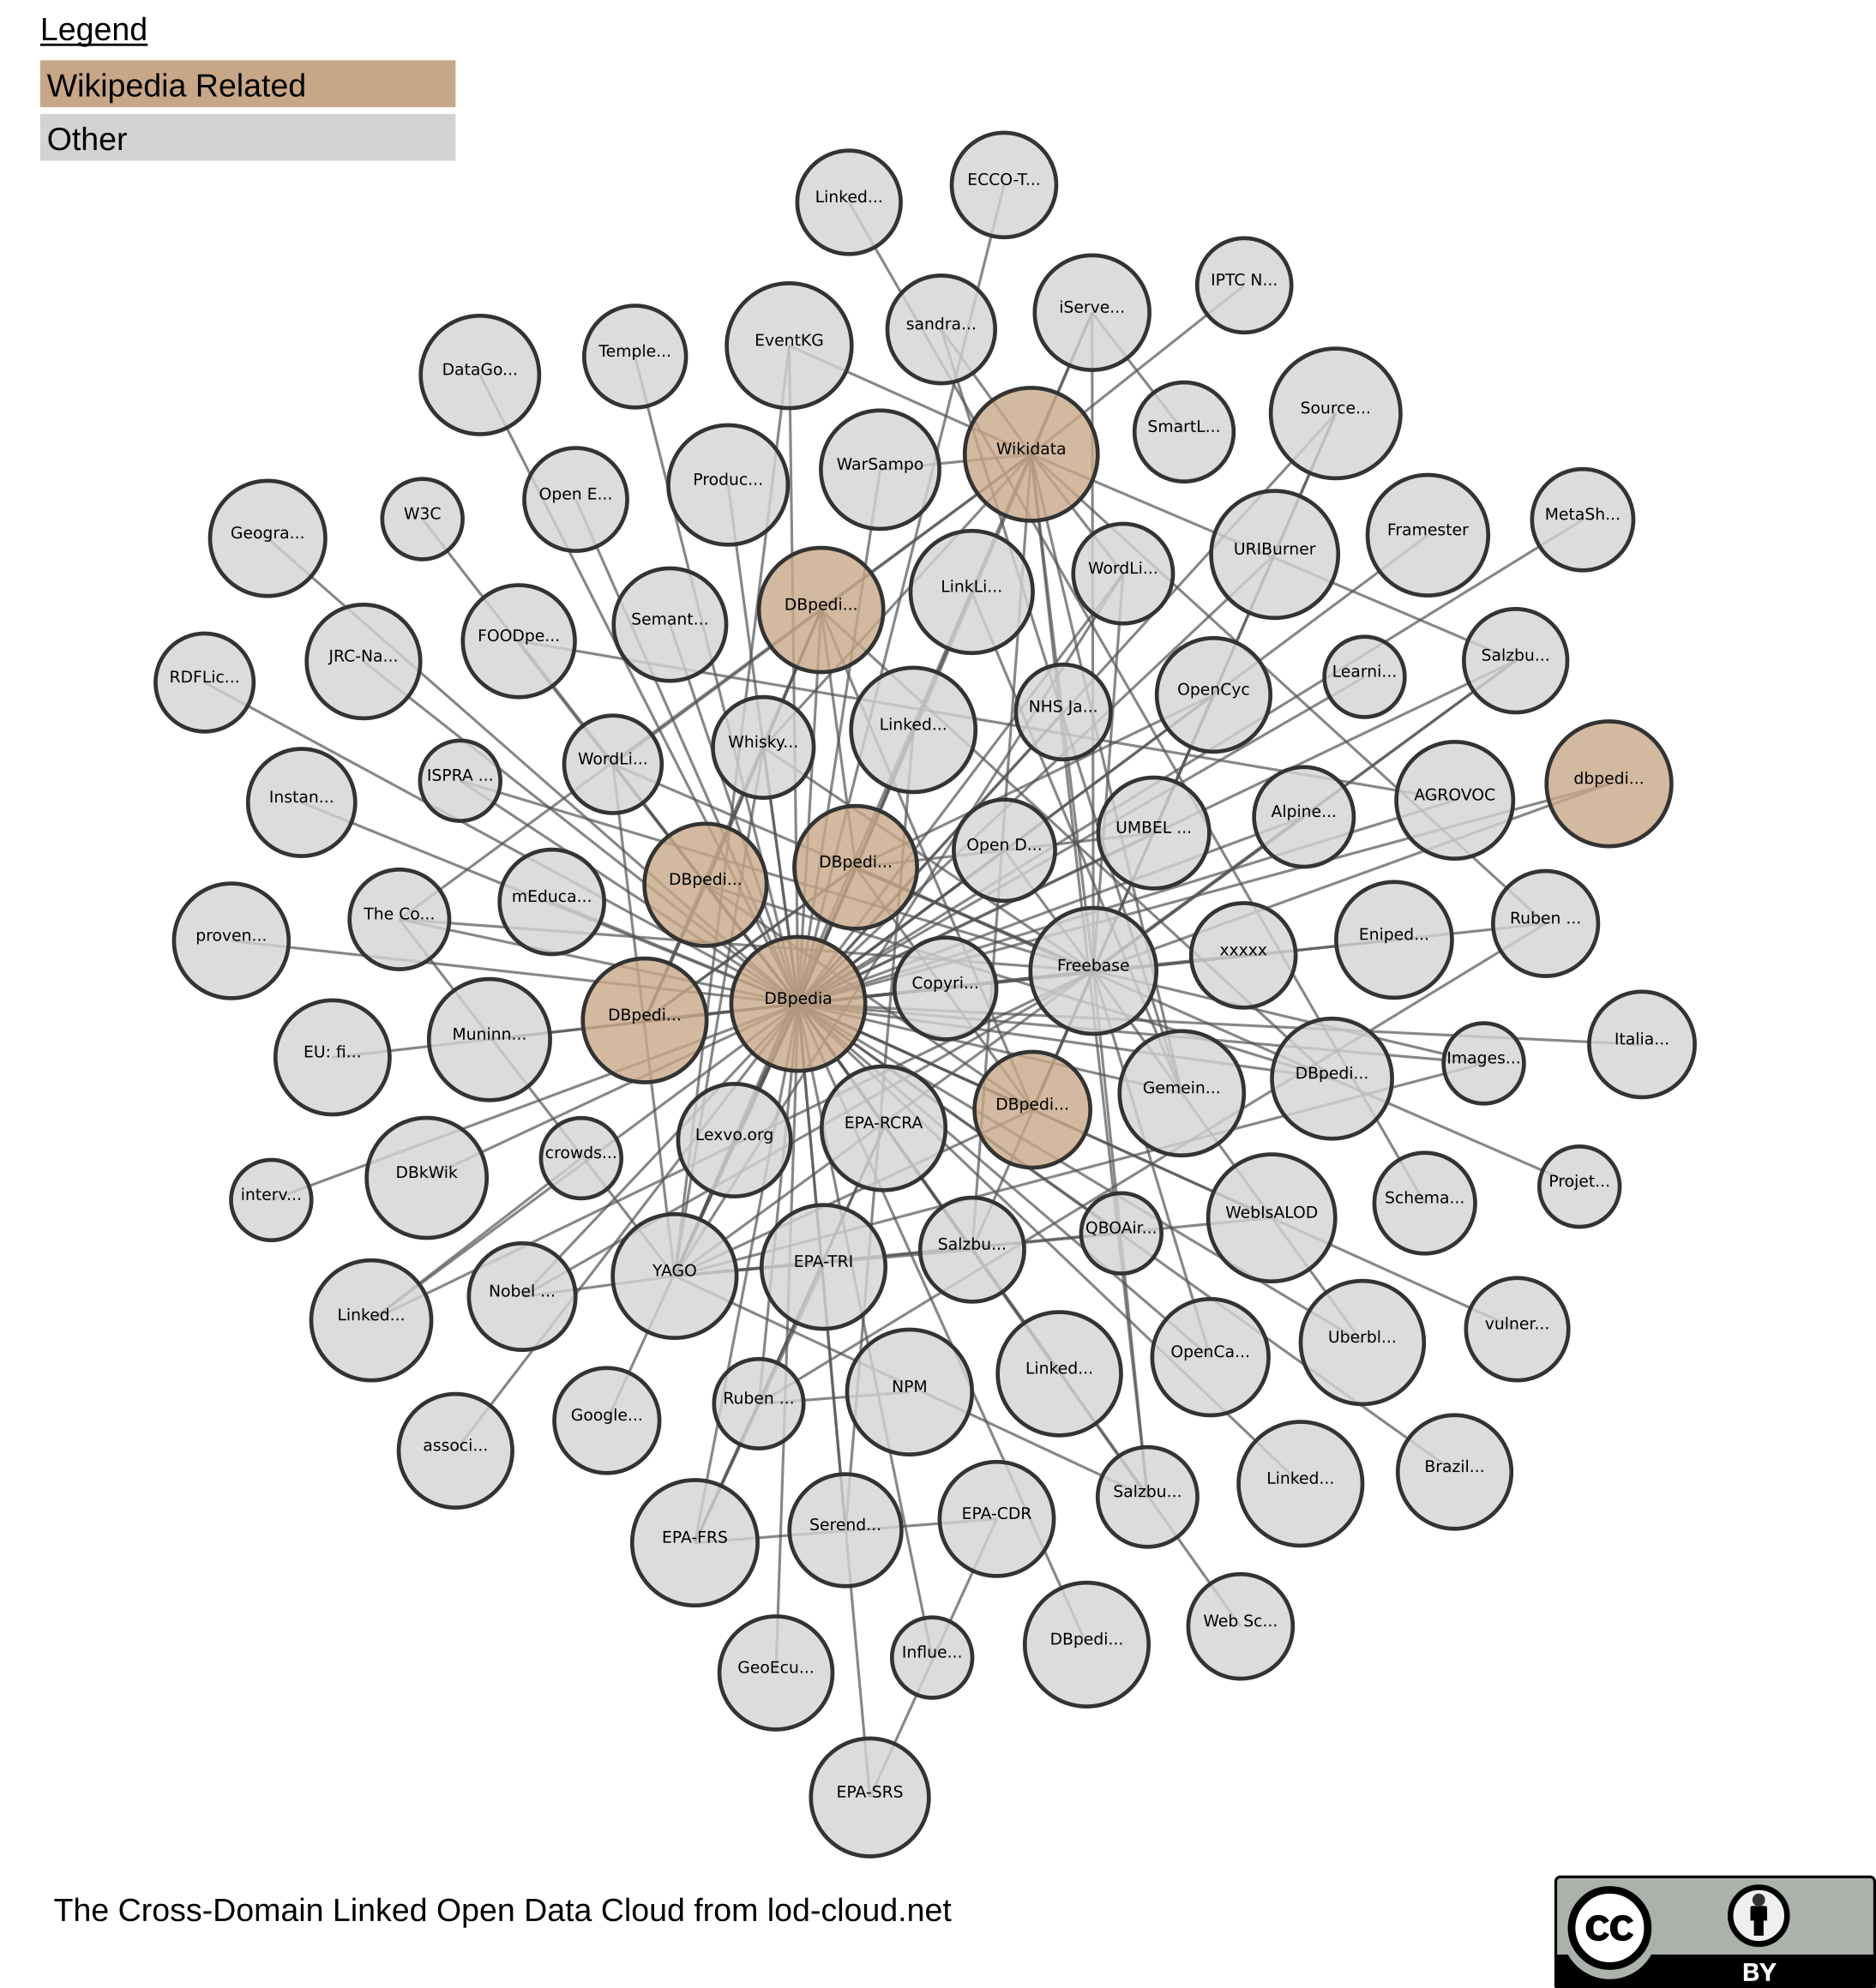
\includegraphics[width=0.8\textwidth]{images/cross-domain-lod.png}
    \caption{Sub-grafo das bases de conhecimento da \textit{Linked-Open-Data}.}
    \label{fig:lod_cloud}
\end{figure}

\subsection{Knowledge Base Completion Techniques}

As técnicas presentes na literatura, cujo propósito é atacar a incompletude das bases de conhecimento, buscam basicamente encontrar os fatos faltantes a partir da análise dos demais. Atualmente, o estado-da-arte nessa tarefa é o que se conhece por \textit{Knowledge Base Embedding}, no qual as entidades e seus relacionamentos são mapeados em um espaço vetorial de baixa dimensão. Desse modo, pode-se inferir, com certo grau de incerteza, relações que antes eram desconhecidas. 

Em (Border et. al 2013)\cite{NIPS2013_5071}, é proposto o método TransE de \textit{Knowledge Embedding}, no qual os relacionamentos são interpretados como translações no espaço vetorial correspondente. Por exemplo, considere o fato ``\textit{Pelé é o rei do futebol}". No espaço gerado pelo TransE, o vetor correspondente à entidade``Pelé" somado à relação ``Rei" deve ser igual ou significantemente próximo à entidade ``Futebol". 

Embora esse método funcione bem para relacionamentos do tipo um a um, isto é, o futebol só pode ter um único rei e o Pelé só é rei de um esporte, e não reflexivas, para os demais casos não apresenta bons resultados.

Para lidar com tais limitações, outros métodos, como o TransH \cite{Wang2014KnowledgeGE}, surgiram com novas abordagens. Nesse caso, cada hiperplano é representado por um hiperplano $w_{r}$ ao invés de um vetor como no TransE. Um fato é verdadeiro no espaço gerado pelo TransH se a distância $d_{r}$ entre as projeções das entidades no plano $w_{r}$ é próxima de zero.
 
\begin{figure}[h]
    \centering
    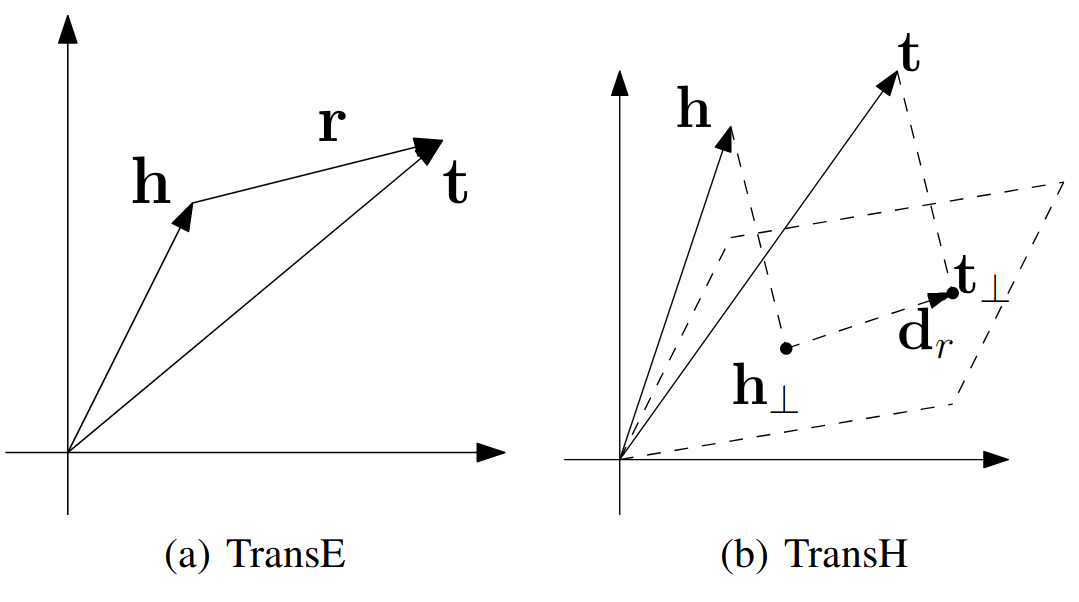
\includegraphics[scale=0.4]{images/TransE-TransH.png}
    \caption{Representações dos modelos TransE e TransH \cite{Wang2014KnowledgeGE}.}
    \label{fig:trasnE_transH}
\end{figure}

\subsection{Explainable Knowledge Embedding (XKE)}

Apesar dos recentes avanços na construção de \textit{Knowledge Base Completion}, apresentados na seção acima, os espaço vetoriais gerados por esses métodos são pobres em termos de interpretabilidade. Esses \textit{embeddings} são particularmente opacos, pois representam entradas ricas de significado de uma forma numérica, em que cada dimensão não carrega nenhum ou pouco sentido. 

Com o intuito de explicar um \texit{Knowledge Base Ebedding}, recentemente foi desenvolvido o método XKE, \textit{Explainable Knowledge Embedding}. Esse método aplica a técnica SFE \textit{Subgraph Feature Extraction} \cite{Gardner-et-al2015} para extrair \textit{features} binárias de um grafo que indicam a existência de um caminho entre dois elementos. A partir desses resultados, são treinadas vários modelos de regressão logística, os quais são interpretáveis.

\section{User Interface}

\subsection{Graphical \& Command Line}

A interação homem-máquina hoje, na maioria dos dispositivos, se dá por meio de elementos visuais, como botões, tabelas, barras, imagens, etc. Esse tipo de interface, conhecido por GUI, tem origem nos anos 70 com o sistema Xerox Alto, num cenário em que a CLI (\textit{Command Line Interface}) era predominante. 

Apesar de muito simples, a CLI exige um conhecimento técnico significativo, o qual cresce em função da quantidade de comandos. Nesse sentido, conforme os sistemas se tornam cada vez mais complexos, mais tempo demora a curva de aprendizado necessária para utilizá-los. Além de que, a medida que os comandos também crescem em complexidade, aumentam os números de parâmetros envolvidos e, consequentemente, a incidência de erros.

A GUI surgiu como alternativa mais intuitiva e de fácil utilização frente a CLI. Embora tenha melhorado a usabilidade e, assim, proporcionado melhor UX (\textit{User Experience}), tornou muito mais complexo o desenvolvimento de uma interface.

\subsection{Conversational}

Essencialmente a GUI moveu a responsabilidade pela complexidade do sistema, a qual era do usuário com a CLI, para o desenvolvedor, o que se traduz em maior custo de projeto. Além de que, por mais intuitivo que seja, a representação baseada em elementos visuais tem suas limitações.

Do mesmo modo que a GUI buscava cobrir as deficiências da CLI, os agentes conversacionais surgem como a nova geração de interface homem-máquina. Com o recente progresso em IA e NLP, hoje é possível computar linguagem natural de forma eficaz. Assim, além de texto ser muito mais flexível do que elementos visuais, o gasto de desenvolvimento é relativamente baixo. 

Pode-se separar os agentes conversacionais em duas categorias: \textbf{Task-Oriented} e \textbf{Chatbots}. Enquanto a primeira contempla aqueles projetados para executar tarefas específicas de domínio fechado, por exemplo reservar uma mesa em um restaurante, em conversas curtas, a segunda visa produzir extensas interações em diferentes contextos. 

\part{Tecnologias Utilizadas}

\chapter{Tecnologias Utilizadas}
\capepigrafe[0.5\textwidth]{``Instrumental or mechanical science is the noblest and, above all others, the most useful.''}{Leonardo da Vinci}

Este trabalho utilizará um diverso conjunto de tecnologias em sua implementação, desde bibliotecas de software até plataformas de computação em nuvem. A princípio os modelos de aprendizado de máquina serão desenvolvidos, sempre que possível, em Python 3.7 com o uso dos \textit{frameworks}: NLTK, Gensim e Tensorflow. O projeto de software do chatbot será implementado em TypeScript na \textit{runtime} NodeJS 6.0. 

\section{NLTK, Tensorflow e Gensim}

Optou-se por utilizar Tensorflow, NLTK e Gensim no desenvolvimento dos modelos de \textit{Machine Learning} utilizados neste projeto. Além de serem bem robustos, esses toolkits são bem completos no sentido de atender as demandas deste projeto.

\section{Dialogflow}

Baseado no estudo comparativo entre os diversos \textit{frameworks} de desenvolvimento de chatbots disponíveis na literatura (IBM Watson, Wit.ai, LUIS, etc) \cite{Correa-et-al-2018}, optou-se por utilizar o Dialogflow neste projeto. A decisão foi tomada em função da acurácia na detecção de intenções, ou seja, sua eficiência em  \textit{Dialog Act Classification}, suporte à linguagem portuguesa (pt-br) e preço. O Dialoflow, além de ser gratuito e ter suporte a treze linguagens inclusive o pt-br, ocupa a segunda posição em termos de acurácia (99,6\%). 

\section{Google Cloud Platform}

Por questões de simplicidade, eficiência e segurança, decidiu-se por usar o serviço completo de BAAS (\textit{Backend As A Service}) Firebase da Google Cloud Plataform, o que inclui Cloud Functions, Firestore e PubSub.

Além de ser gratuita, para as demandas deste projeto, oferece ampla variedade de serviços e métricas pertinentes (latência, registro de transações, etc).

\section{OpenKE}

O OpenKE é um \textit{toolkit} open-source que proporciona um \textit{framework} unificado e vários modelos para a geração de \textit{Knowledge Embeddings} (TransE, TransH, etc) \cite{D18-2024}. Esse pacote, além de ter suporte para Tensorflow, possibilita a utilização de GPU, o que é fundamental dada a grande quantidade de poder computacional necessária para treinar esses \textit{embeddings}. 

\begin{figure}[h]
    \centering
    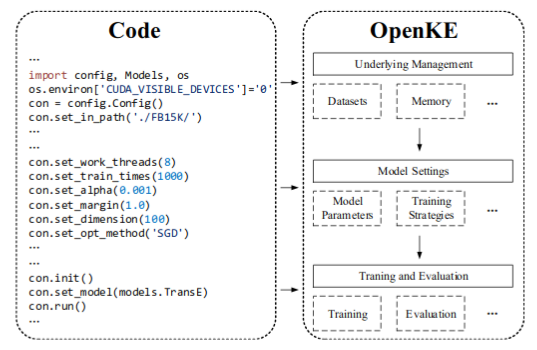
\includegraphics[scale=0.5]{images/openKE.png}
    \caption{Um exemplo de treinamento de um KE (TransE) com OpenKE \cite{D18-2024}.}
    \label{fig:trasnE_transH}
\end{figure}

\part{Metodologia de Trabalho}

\chapter{Metodologia de Trabalho}
\capepigrafe[0.5\textwidth]{``To achieve great things, two things are needed: a plan, and not quite enough time.''}{Leonard Bernstein}

A metodologia adotada neste trabalho será baseada em outros casos de estudo presentes na literatura de chatbots \cite{Musto-et-al} \cite{Correa-et-al-2018}. Nesse sentido, adotará uma abordagem \textit{user centered design}, a qual se apoia no tripé: comportamento do usuário, métricas empíricas e desenvolvimento interativo \cite{Gould:1983:DUP:800045.801579}.

\section{Desenvolvimento}

Pretende-se seguira a arquitetura tradicional de chatbots, que inclusive já foi utilizada pelo projeto de referência \cite{Correa-et-al-2018}. A arquitetura consiste em um módulo de interação com o usuário, um de processamento de linguagem natural e um de consulta. O módulo de NLP faz a análise sintática e morfológica das entradas, com uso de aprendizado de máquina para melhora de desempenho, por fim o de consulta é específico da aplicação. Haverá a necessidade de se inserir um novo módulo, de geração de explicações, o qual atuará intimamente com o de consulta.

Uma vez construído e integrado o módulo de geração de explicações ao chatbot, o sistema será testado. No contexto deste trabalho, o primeiro ponto será verificar qual a acurácia em identificar perguntas que exigem uma explicação. Para tanto, serão realizadas sessões com usuários do próprio grupo de pesquisa, e com estudantes da Escola Politécnica que são usuários comuns do sistema Júpiter e estão inseridos em um processo educacional. Além da medida objetiva de acurácia, será necessário também avaliar a qualidade das explicações em si. 

A metodologia de avaliação será a mesma emprega em trabalhos correlatos e de acordo com as diretrizes na literatura \cite{Correa-et-al-2018}. A análise de usabilidade de chatbots tem recebido bastante atenção, com destaque para esquemas como BLEU e PARADISE cujo propósito é verificar o quanto uma resposta tem sobreposição significativa com a resposta pretendida \cite{Walker:1997:PFE:979617.979652}.

\section{Planejamento}

O planejamento de execução doste trabalho pode ser descrito, de forma resumida, nas seguintes atividades:

\begin{enumerate}
    \item Revisão da literatura sobre chatbots. Será em particular estudado o pacote Dialogflowe a arquitetura do JupiterwebChatbot.
    \item Revisão da literatura sobre interpretabilidade e geração de explicação. Além da análise bibliométrica da literatura sobre chatbots.
    \item Projeto do módulo de geração de explicações, de recomendação e de \textit{Question-Answering} para o chatbot. 
    \item Implementação dos módulos, com ênfase na geração de explicações.
    \item Teste de acurácia e usabilidade do módulo de geração de explicações.
    \item Escrita de relatórios e documentação.
\end{enumerate}

Estas atividades serão organizadas como segue, distribuídas nos doze meses:

\begin{figure}[h]
    \centering
    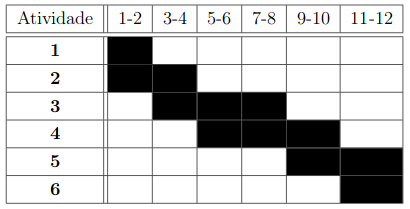
\includegraphics[width=0.75\textwidth]{images/roadmap.png}
    \caption{\textit{Roadmap} resumido do projeto.}
    \label{fig:project_roadmap}
\end{figure}

\part{Especificação de Requisitos do Sistema}

\chapter{Especificação de Requisitos do Sistema}
\capepigrafe[0.5\textwidth]{``Everything is designed. Few things are designed well.''}{Brian Reed}

\section{Requisitos Não Funcionais}

\subsection{Desempenho}

O desempenho do chatbot pode ser entendido como a sua capacidade de identificar corretamente as intenções do usuário por meio de uma classificação multi-classe, em que \textit{feature} estaria associada com uma classe correspondente. 

A abordagem tradicionalmente adotada na avaliação de classificadores é a análise da matriz de confusão, a qual relaciona a classificação de cada elemento com seu real valor. Assim, é possível obter métricas que ajudam em medir a qualidade do diálogo. Por exemplo, considere a matriz de confusão abaixo:

\begin{figure}[h]
    \centering
    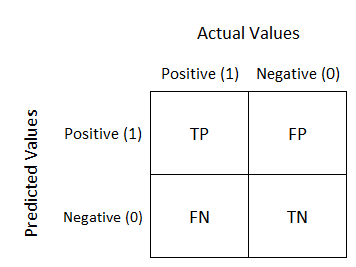
\includegraphics[width=0.7\textwidth]{images/confusion-matrix.png}
    \caption{Exemplo de matriz de confusão binária.}
    \label{fig:project_roadmap}
\end{figure}

A partir dessa matriz, pode-se extrair cinco métricas da performance do classificador \cite{Hossin-Sulaiman-2015}.

\begin{table}[h!]
  \begin{center}
    \begin{tabular}{l|c|p{8cm}}
      \textbf{Métrica} & \textbf{Fórmula} & \textbf{Descrição}\\
      \hline
       & & \\
      Accuracy (acc) & $\frac{TP+TN}{TP+TN+FP+FN}$ & Razão de classificações corretas sobre total \\
       & & \\
      Error rate (err) & $1-acc$ & Razão de classificações incorretas sobre total\\
       & & \\
      Precision (p) & $\frac{TP}{TP+FP}$ & Probabilidade de uma classificação positiva ser de fato positiva\\
       & & \\
      Recall (r) & $\frac{TP}{TP+FN}$ & Probabilidade de uma entrada positiva ser classificada como tal\\
       & & \\
      F1-Score & $2*\frac{p*r}{p+r}$ & Média harmônica entre \textit{precision} e \textit{recall}\\
    \end{tabular}
    \caption{Métricas de avaliação de performance.}
    \label{tab:table1}
  \end{center}
\end{table}

Para este trabalho, assume-se como requisitos de performance para todas as classes: acurácia maior ou igual a \textbf{96\%}, precisão maior ou igual a \textbf{95\%}, \textit{recall} e \textit{f1-score} maiores ou iguais a \textbf{90\%}. Tais valores foram baseados em resultados similares na literatura \cite{Correa-et-al-2018}.

\subsection{Usabilidade}

A usabilidade do sistema configura um de seus requisitos mais importantes. Além de utilizar pesquisas de opinião com estudantes e pesquisadores, será utilizado o \textit{framework} PARADISE (\textit{PARAdigm for DIalog System Evaluation}) \cite{Walker:1997:PFE:979617.979652} para a avaliação de usabilidade. Ao contrário de métodos mais simples como o BLEU \cite{Papineni02bleu:a}, que medem a sobreposição das respostas com aquelas consideradas como verdadeiras, o PARADISE trabalha com diversos fatores que contribuem para a satisfação do usuário, como duração da conversa, \textit{task success rate} e incidência de erros. 

A partir desses critérios, espera-se obter resultados superiores aos apresentados em trabalhos anteriores \cite{Correa-et-al-2018}.

\section{Especificação Funcional}

Além das \textit{features} especificadas no projeto de referência, como buscar e sugerir informações de uma disciplina \cite{Correa-et-al-2018}, será desenvolvido o módulo de explicações e o de \textit{Question-Answering}. Esta parte contempla a especificação desses dois novos módulos, além da melhoria do sistema de recomendação.

\begin{table}[h]
\centering
\begin{tabular}{|p{6cm}|p{8cm}|}
\hline
\multicolumn{1}{|c|}{\textbf{Objetivo}}                                                    & \multicolumn{1}{c|}{\textit{\textbf{Feature}}}      \\ \hline
\multirow{Buscar informações de uma disciplina de escolha}                  & Fornecer descrição de disciplina           \\ \cline{2-2} 
                                                                                  & Fornecer os professores responsáveis       \\ \cline{2-2} 
                                                                                  & Fornecer os horários de oferecimento       \\ \cline{2-2} 
                                                                                  & Informar os requisitos da disciplina       \\ \cline{2-2} 
                                                                                  & Fornecer a quantidade de créditos          \\ \cline{2-2} 
                                                                                  & Fornecer a carga-horária da disciplina     \\ \hline
\multirow{Sugerir disciplinas a partir dos critérios de interesse do aluno} & Sugerir curso por tema de interesse        \\ \cline{2-2} 
                                                                                  & Sugerir curso por preferência de professor \\ \cline{2-2} 
                                                                                  & Sugerir com restrição de horário           \\ \hline
\multirow{Sugerir materiais de estudo a partir do interesse do aluno}       & Sugerir artigo por tema de interesse       \\ \cline{2-2} 
                                                                                  & Sugerir artigo por similaridade com outro  \\ \cline{2-2} 
                                                                                  & Explicar recomendação                      \\ \hline
\multirow{Elucidar dúvidas pertinentes ao processo de aprendizado do aluno} & Responder perguntas sobre conteúdos        \\ \cline{2-2} 
                                                                                  & Explicar respostas                         \\ \hline
\end{tabular}
\caption{Tabela de \textit{Features} do sistema.}
\label{my-label}
\end{table}

% ========== Referências ==========
% --- IEEE ---
%	http://www.ctan.org/tex-archive/macros/latex/contrib/IEEEtran
%\bibliographystyle{IEEEbib}

% --- ABNT (requer ABNTeX 2) ---
%	http://www.ctan.org/tex-archive/macros/latex/contrib/abntex2
\bibliographystyle{abntex2-num}

\bibliography{references}

% ========== Apêndices (opcional) ==========
%\apendice
%\chapter{}
%\chapter{Beta}


% ========== Anexos (opcional) ==========
\anexo
\chapter{Jupiterweb Chatbot}

\section{Diagramas de Estados}

\begin{figure}[h]
    \centering
    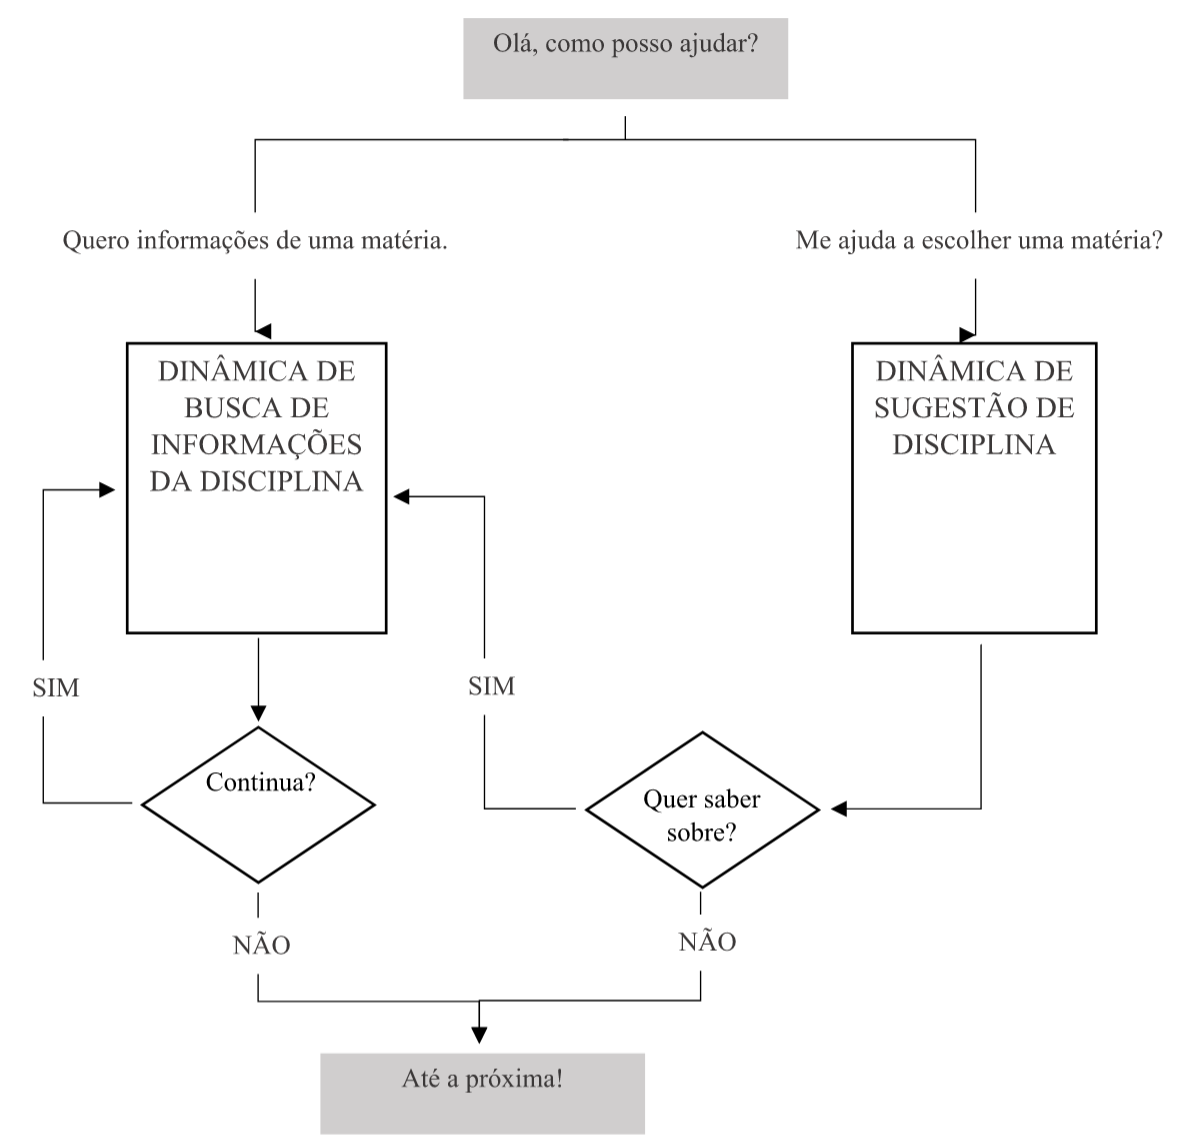
\includegraphics[width=1\textwidth]{images/anexo/asm-general.png}
    \caption{Estrutura geral de diálogo do Jupiterweb Chatbot.}
    \label{fig:asm_general}
\end{figure}

\begin{figure}[h]
    \centering
    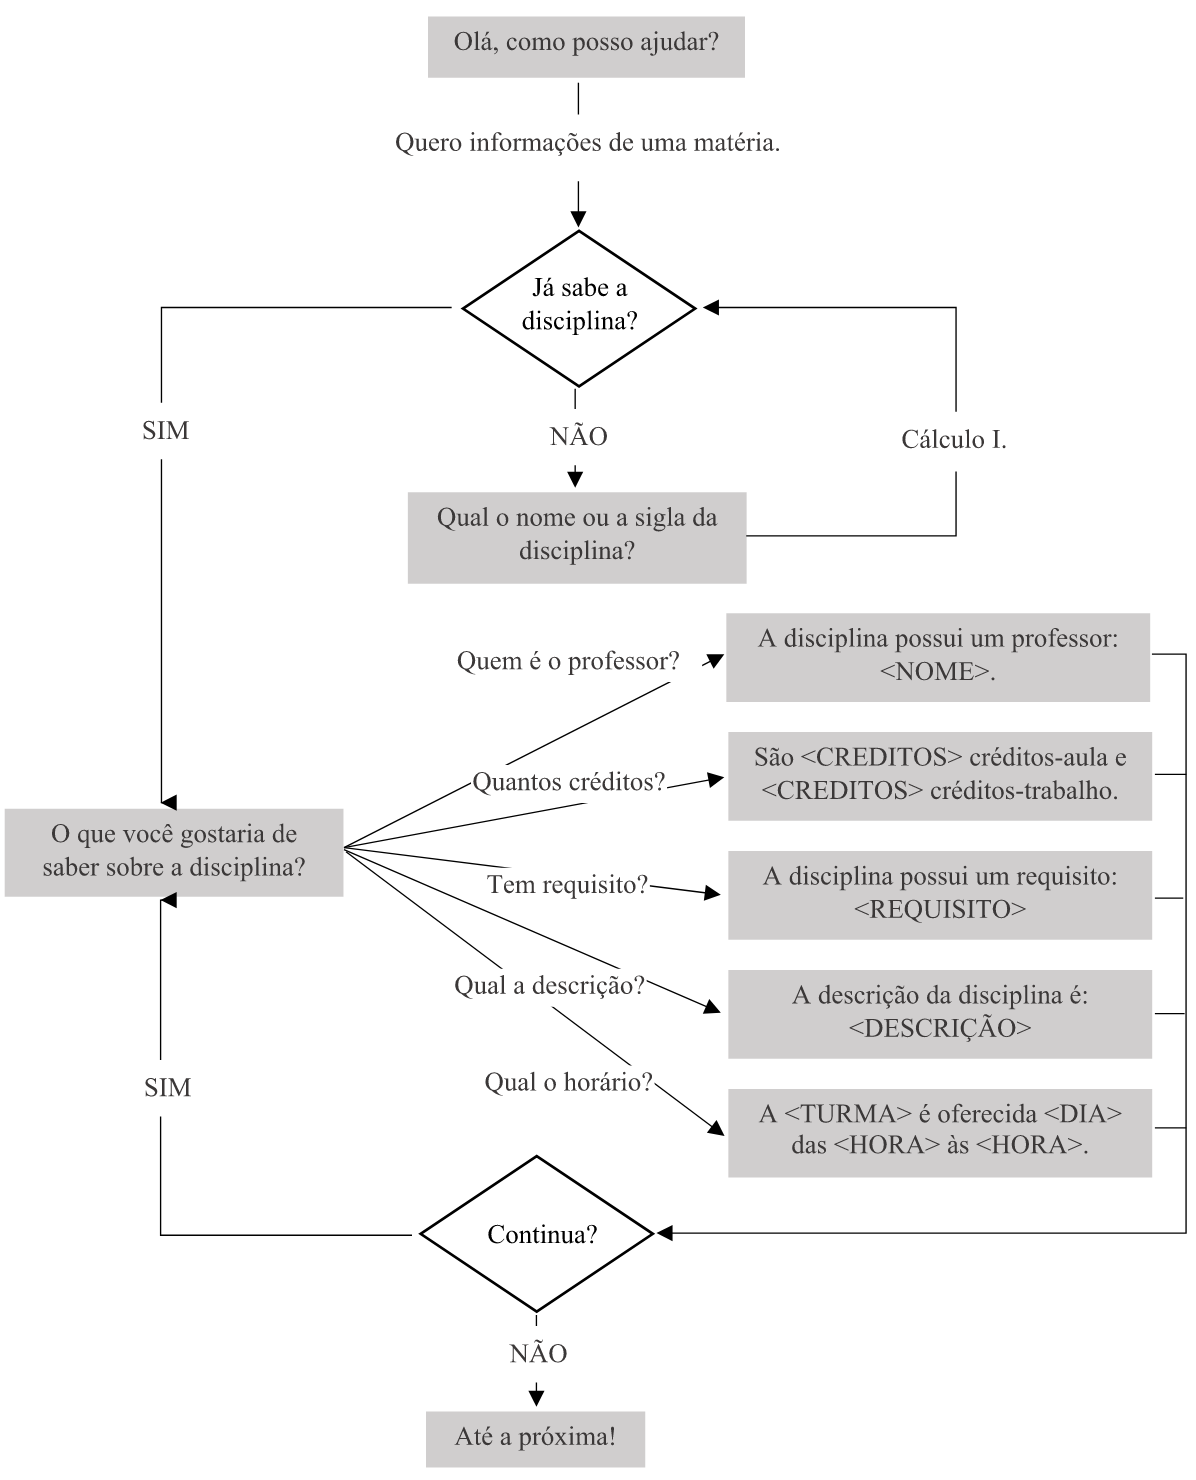
\includegraphics[width=1\textwidth]{images/anexo/asm-query.png}
    \caption{Estrutura do diálogo do caso de uso \textit{Buscar Informações de Disciplina}.}
    \label{fig:asm_query}
\end{figure}

\begin{figure}[h]
    \centering
    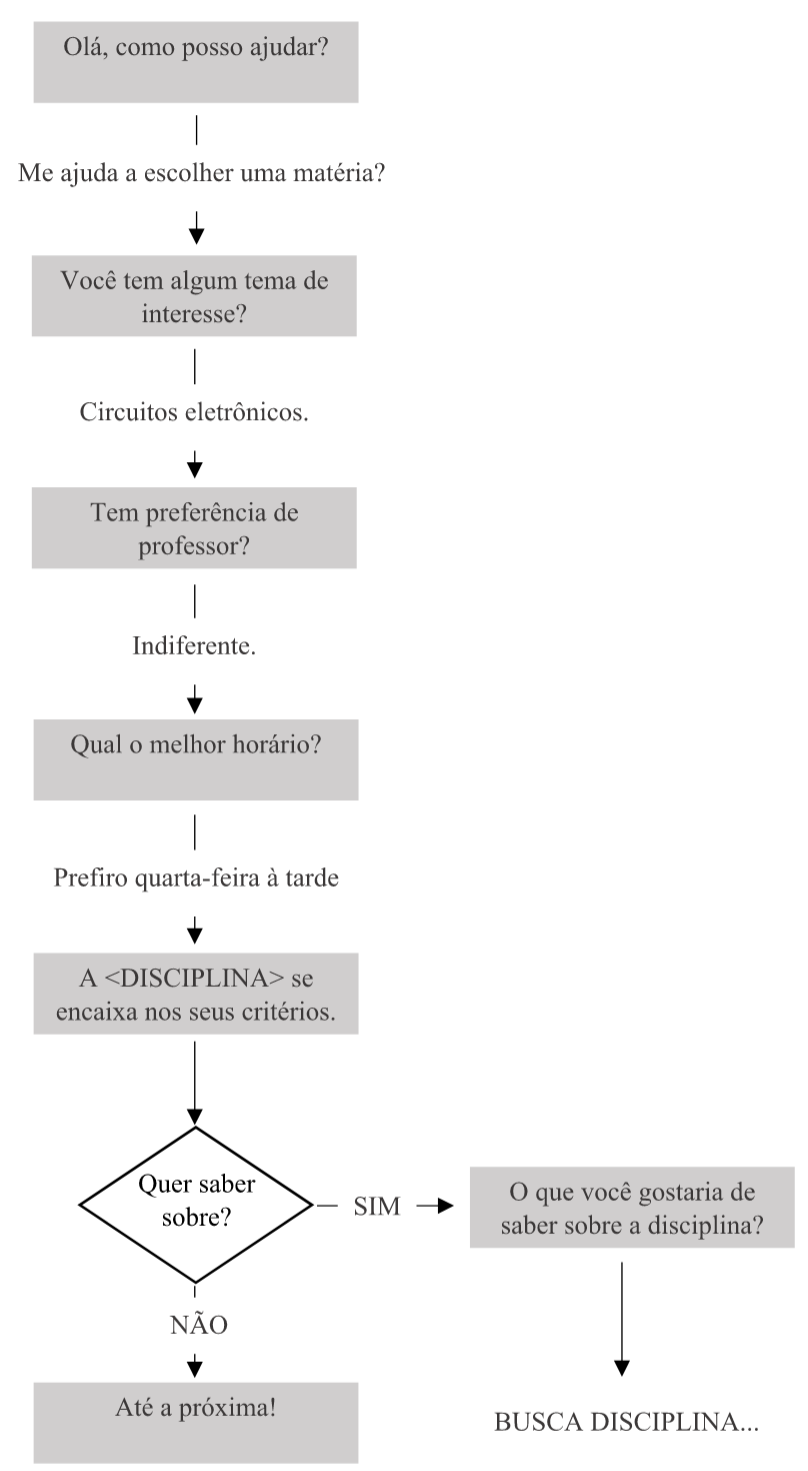
\includegraphics[width=0.8\textwidth]{images/anexo/asm-suggestion.png}
    \caption{Estrutura do diálogo do caso de uso \textit{Sugerir Disciplina}.}
    \label{fig:asm_recommendation}
\end{figure}




\end{document}
